\documentclass[11pt, twoside, a4paper]{article}
\usepackage[italian]{babel}
\usepackage[utf8]{inputenc}
\usepackage{amsmath}
\usepackage{fullpage}
\usepackage{graphicx}
\usepackage{booktabs}
\usepackage{wrapfig}
\usepackage{sidecap}

\begin{document}

\begin{titlepage}
\begin{center}
	\hrule \vspace{0.5cm}
     	\textsc{\LARGE Misure ripetute di lunghezza e tempo}
	\vspace{0.5cm} \hrule \vspace{2cm}
      	{\large Francesco Pasa, Davide Bazzanella, Andrea Miani\\
		Gruppo A11}\\
	\vspace{0.5cm}
      	{\large 28 febbraio 2013 - 11 marzo 2013}
	\vfill
	{\begin{abstract}
Misura della lunghezza di un gruppo di 25 cilindri di metallo e della durata del periodo di oscillazione di un pendolo semplice.
Analisi dei valori ottenuti dagli esperimenti del singolo gruppo e dei valori raccolti dagli esperimenti di tutti i gruppi di laboratorio.
	 \end{abstract}}
\end{center}
\end{titlepage}

\newpage

\vspace*{\fill}
\begin{center}
	\tableofcontents
\end{center}
\vspace*{\fill}

\newpage

\section{Introduzione}
Questa relazione sarà divisa in due sezioni, una dedicata al primo esperimento
in cui verrà misurata la lunghezza di una popolazione di 25 cilindri metallici
con tre diversi strumenti (metro a nastro, calibro ventesimale, micrometro).
L'altra dedicata alla misura del periodo di un pendolo semplice (costruito con
un cavo inestensibile e un peso) effettuata da tutti i componenti del gruppo
al fine di evidenziare la presenza di eventuali errori sistematici, dovuti
alla differente prontezza di riflessi dei componenti dell'equipe. Entrambe
le sezioni saranno integrate con l'analisi dei dati ottenuti dagli
esperimenti, in particolare la prima conterrà anche lo studio dei dati
ottenuti da tutti gli altri gruppi del corso di laboratorio.

\section{Cilindretti}

\subsection{Descrizione della procedura di misura}
Procediamo ora con la descrizione della procedura operativa con cui
abbiamo misurato i 25 cilindri di metallo con i tre strumenti di
misura a nostra disposizione:

\subsubsection{Metro a nastro}
Abbiamo misurato i 25 cilindretti con un metro a nastro la cui risoluzione
di misura è 1 millietro, in quanto abbiamo ritenuto di non poter distinguere
un intervallo di mezzo millimetro. Per questo motivo abbiamo approssimato
le misure alla tacca da un millimetro più vicina al bordo del cilindretto.
Poichè la lunghezza dei cilindretti era di circa 15 mm abbiamo incontrato
delle difficoltà nell'allineare i cilindri con lo 0 dello strumento.
Per questo motivo abbiamo allineato un'estremità di ogni cilindro con la
tacca dei 10 cm del metro e abbiamo sottratto questa quantità al valore
della misurà così ottenuta. E' importante evidenziare che in questa
operazione abbiamo riscontrato una difficoltà nell'allineare correttamente
i cilindri anche con la tacca dei 10 cm, inoltre abbiamo tentato di evitare
eventuali errori di parallasse durante la lettura dello stumento.

\subsubsection{Calibro ventesimale}
Il calibro che abbiamo utillizzato ha una risoluzione di misura di 0.05
millimetri. La misura con il calibro ventesimale è stata effettuata avendo
cura di disporre i cilindri in modo perpendicolare ai becchi del calibro.
[In questo modo abbiamo tentato di misurare l'asse del cilindro e non una
sua proiezione], a tal fine abbiamo sfruttato le scanalature presenti sullo
strumento; tuttavia non abbiamo potuto evitare nella maniera più assoluta
errori di questo tipo.
La lettura dei ventesimi di millimetro è stata effettuata cercando quale
tacca della scala mobile ventesimale si allineasse meglio con le tacce
sovrastanti della scala millimetrata. Questa operazione è stata eseguita
da tutti i membri del gruppo per evitare eventuali problemi di parallasse
dovuti ad una singola valutazione della misura.

\subsubsection{Micrometro}
Il micrometro è uno strumento con una risoluzione di misura di 0.01
millimetro. Anche in questo caso la misura dei cilindri è stata effettuata
prestando attenzione che i campioni fossero perpendicolari alle aste di
misurazione, per evitare lo stesso tipo di errore descritto sopra.
Come nel caso del calibro non possiamo essere sicuri del perfetto
allineamento dei cilindri, ma abbiamo tentato di ridurre al minimo
questo "handicap" [questa problematica].

\begin{table}[tb]
	\footnotesize
	\centering
	\begin{tabular} { c c c c c | c c c c c | c c c c c }
		\toprule
		\multicolumn{15}{c}{Lunghezza dei cilindretti} \\
		\multicolumn{5}{c}{Metro [mm]} & \multicolumn{5}{c}{Calibro [mm]} & \multicolumn{5}{c}{Micrometro [mm]} \\
		\midrule
		14 & 14 & 14 & 14 & 14 & 13.70 & 13.85 & 13.95 & 13.80 & 13.95 & 13.94 & 13.92 & 13.84 & 13.93 & 13.79 \\
		14 & 14 & 14 & 14 & 14 & 13.70 & 13.95 & 13.90 & 13.90 & 13.90 & 13.94 & 13.93 & 13.89 & 13.92 & 13.91 \\
		14 & 14 & 14 & 14 & 14 & 13.70 & 13.95 & 13.90 & 13.95 & 13.85 & 13.93 & 13.93 & 13.84 & 13.90 & 13.74 \\
		14 & 14 & 14 & 14 & 14 & 13.70 & 13.95 & 13.90 & 13.90 & 13.90 & 13.70 & 13.85 & 13.91 & 13.79 & 13.70 \\
		13 & 14 & 14 & 14 & 14 & 13.75 & 13.90 & 13.80 & 13.85 & 13.90 & 13.71 & 13.92 & 13.91 & 13.94 & 13.70 \\
	\bottomrule
	\end{tabular}
	\caption{Misure della lunghezza dei 25 cilindretti ottenute con i tre strumenti a nostra disposizione.
        È riportato il valore di lettura degli strumenti.}
\end{table}

\subsection{Analisi dei dati}
La seguente tabella (Tabella 1) riporta tutte le 25 misure di lunghezza
dei cilindri effettuate con i tre strumenti a nostra disposizione:

L'istogramma (Figura 1) rappresenta la distribuzione della lunghezza della
popolazione dei cilindretti ottenuta con il metro a nastro. Per costruire
questo istogramma abbiamo deciso di utilizzare come binnaggio la risoluzione
di misura dello strumento e quindi di 1 millimetro, poichè tutte le misure
effettuate sono risultate essere 14 $\pm$ 0.5 mm tranne una che ha valore
13 $\pm$ 0.5 mm. Come si può osservare dal grafico non siamo riusciti ad
apprezzare la distribuzione non uniforme della lunghezza dei cilindri,
in quanto la risoluzione dello strumento non è stata sufficiente per
apprezzare le variazioni di lunghezza da un corpo all'altro.

\begin{SCfigure}[0.6][bt]
	\centering
	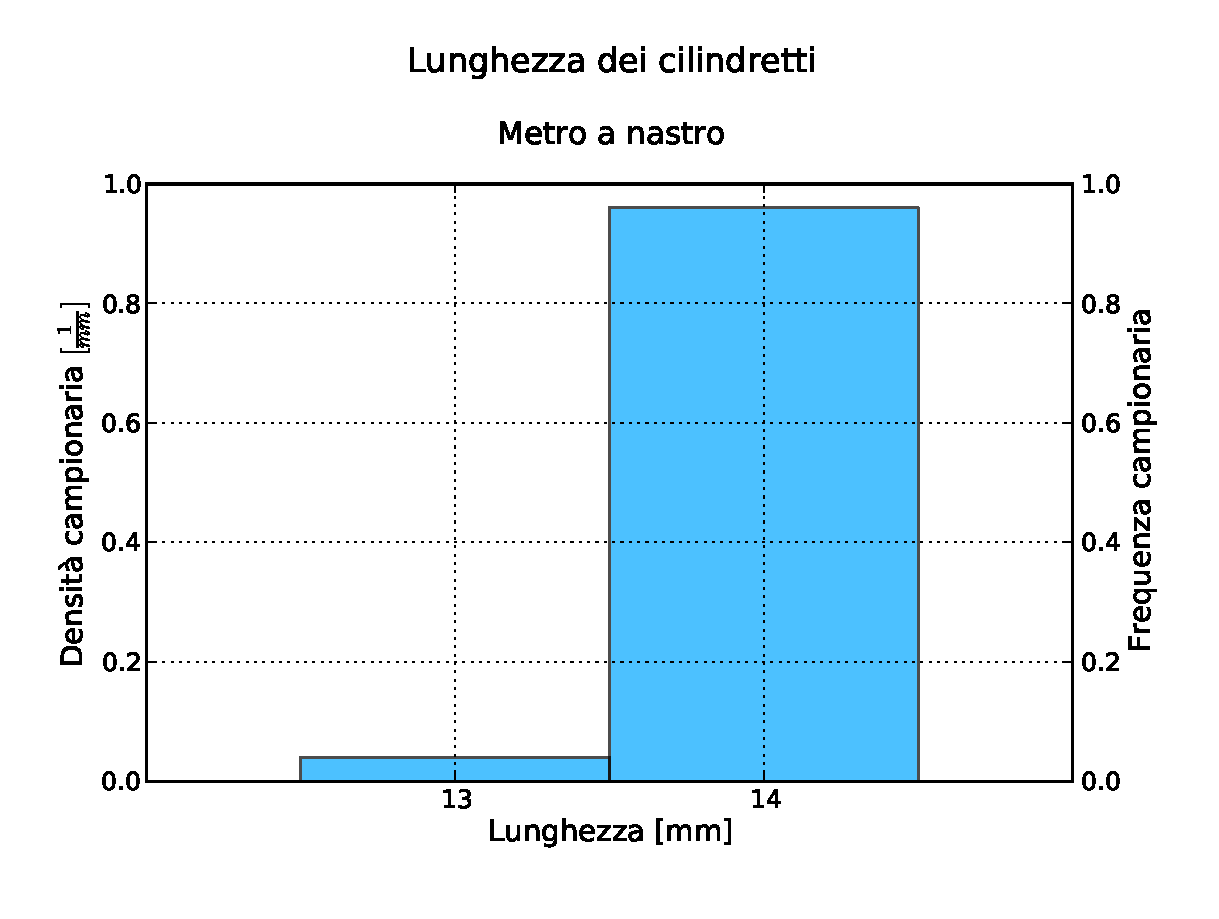
\includegraphics[width=100mm]{Cilindretti_metro.pdf}
	\caption{Istogramma relativo alle misure di lunghezza dei cilindri con il metro a nastro}
\end{SCfigure}

I parametri statistici ottenuti relativi alle misure dei cilindri sono
i seguenti:

% se vuoi elenco numerato sostituisci enumerate al posto di itemize
% ovviemente devi cambiare anche \end{itemize}
\begin{itemize}
    \item{Media campionaria:}
        \begin{equation}
        m^*[x] = \frac{1}{N} \sum_{i=1}^{N} (x_i) \simeq \sum_{j=1}^{\mathcal{N}} (x_j p_j^*) = 13.96\,\,mm 
        \end{equation}

    \item{Varianza campionaria:}
        \begin{equation}
        \tilde{D} = \frac{1}{N - 1} \sum_{i=1}^{N} (x_i - m^*[x])^2 = 0.04\,\,mm^2
        \end{equation}

    \item{Deviazione standard campionaria:}
        \begin{equation}
        \tilde{\sigma} = \sqrt{\frac{1}{N - 1} \sum_{i=1}^{N} (x_i - m^*[x])^2} = 0.2\,\,mm
        \end{equation}
\end{itemize}

Gli istogrammi Figura 2 rappresentano rispettivamente la distribuzione delle
misure della lunghezza dei cilindri ottenute con il calibro ventesimale e con
il micrometro.

\begin{wrapfloat}{figure}{r}{0pt}
	\centering
	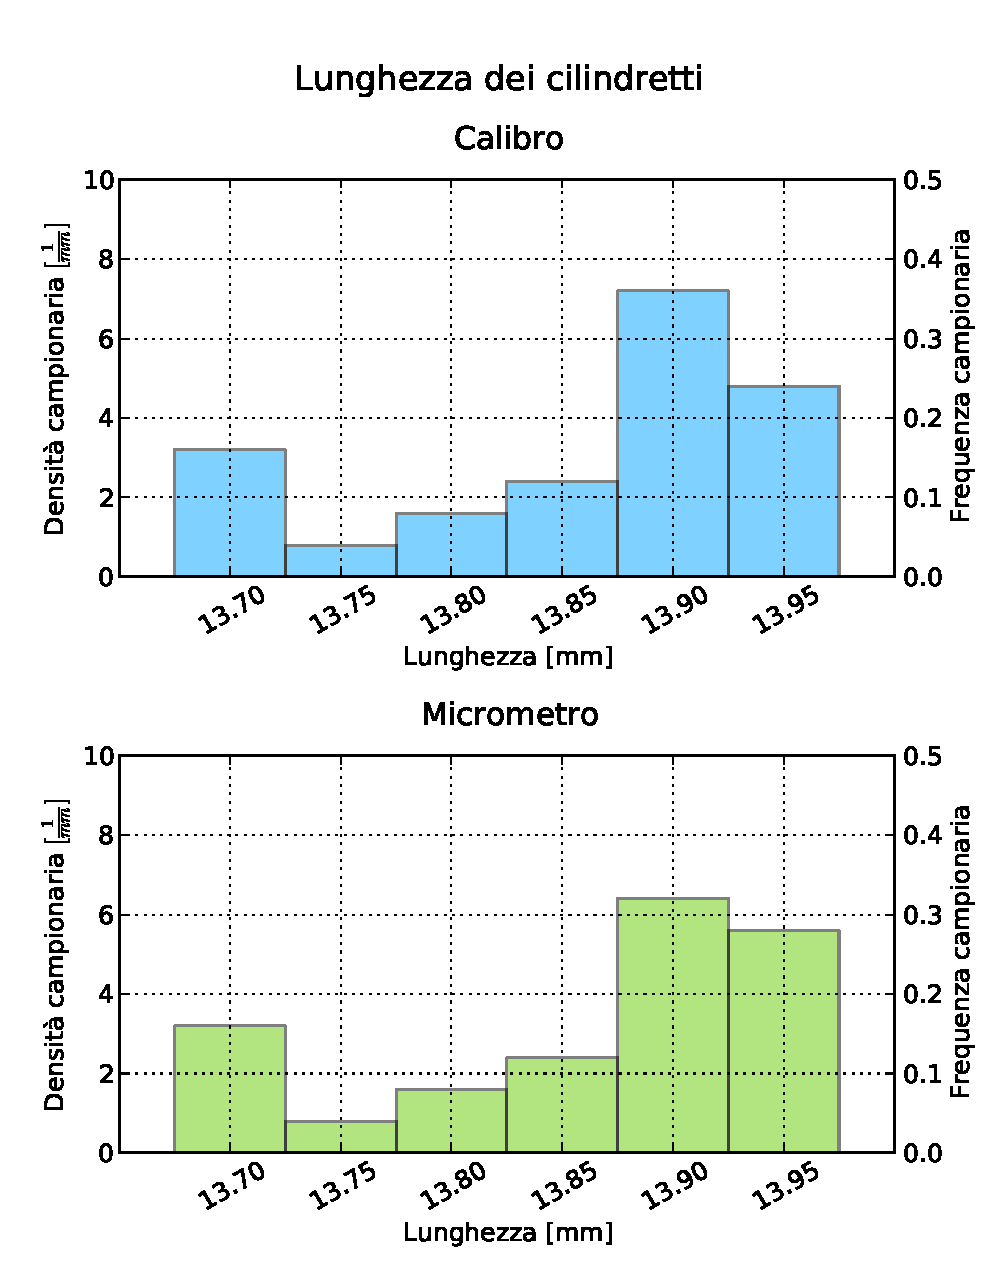
\includegraphics[width=100mm]{Cilindretti_calibro_micrometro.pdf}
	\caption{Istogrammi relativi alle misure di lunghezza dei cilindri con il calibro e con il micrometro}
\end{wrapfloat}

Per l'istogramma relativo al calibro ventesimale la scelta del binning è legata
alla risoluzione dello strumento e quindi la larghezza di ogni singolo
bin è di 0.05 mm. Infatti grazie a questo binnaggio abbiamo un numero
conteggi sufficienti per ogni colonna.

Per l'istogramma relativo al micrometro si è scelto di utilizzare lo stesso
binnaggio utilizzato per il calibro poiché: se avessimo diminuito la larghezza
dei bin avremmo ottenuto un numero di colonne troppo alto e per ognuna di
esse un numero di conteggi insufficiente. Al contrario se avessimo scelto
di aumentare la larghezza dei bin allora lo scopo di misurare i 25 cilindretti
con il micrometro sarebbe risultato vano in quanto non si sarebbe nemmeno apprezzata
la buona risoluzione dello strumento.

Come si può notare i due istogrammi si assomigliano: infatti in entrambi i casi
siamo riusciti ad apprezzare la presenza di un picco della popolazione in
corrispondenza del valore 13.90 mm. Nonostante le misure risultino essere
più accurate rispetto a quelle eseguite con il metro a nastro non ci sono
abbastanza campioni per poter affermare l'esistenza di due popolazioni di
cilindri differenti in quanto l'altro picco, quello riferito al valore ... ,
non è distinguibile da una coda relativa al picco preponderante. Affermiamo
questo perchè l'errore [sulla colonna] è $\sqrt{n_j}$ e il numero di campioni
per questa misura risulta essere inferiore a 5.

Più nel dettaglio possiamo dire che la media campionaria relativa all'istogramma
(1.2) è la seguente: ...
la varianza campionaria risulta essere: ... e la fluttuazione standard campionaria
ottenuta è: ...
Per l'istogramma (1.3) abbiamo ottenuto che la media campionaria risulta essere: ...
la varianza campionaria é: ... e la fluttuazione standard campionaria ottenuta è: ...
% Inserire oltre  a Media campionaria, Varianza campionaria, Fluttuazione standard
% campionaria anche mediana e quantili
% Ulteriori commenti

\begin{SCfigure}
	\centering
	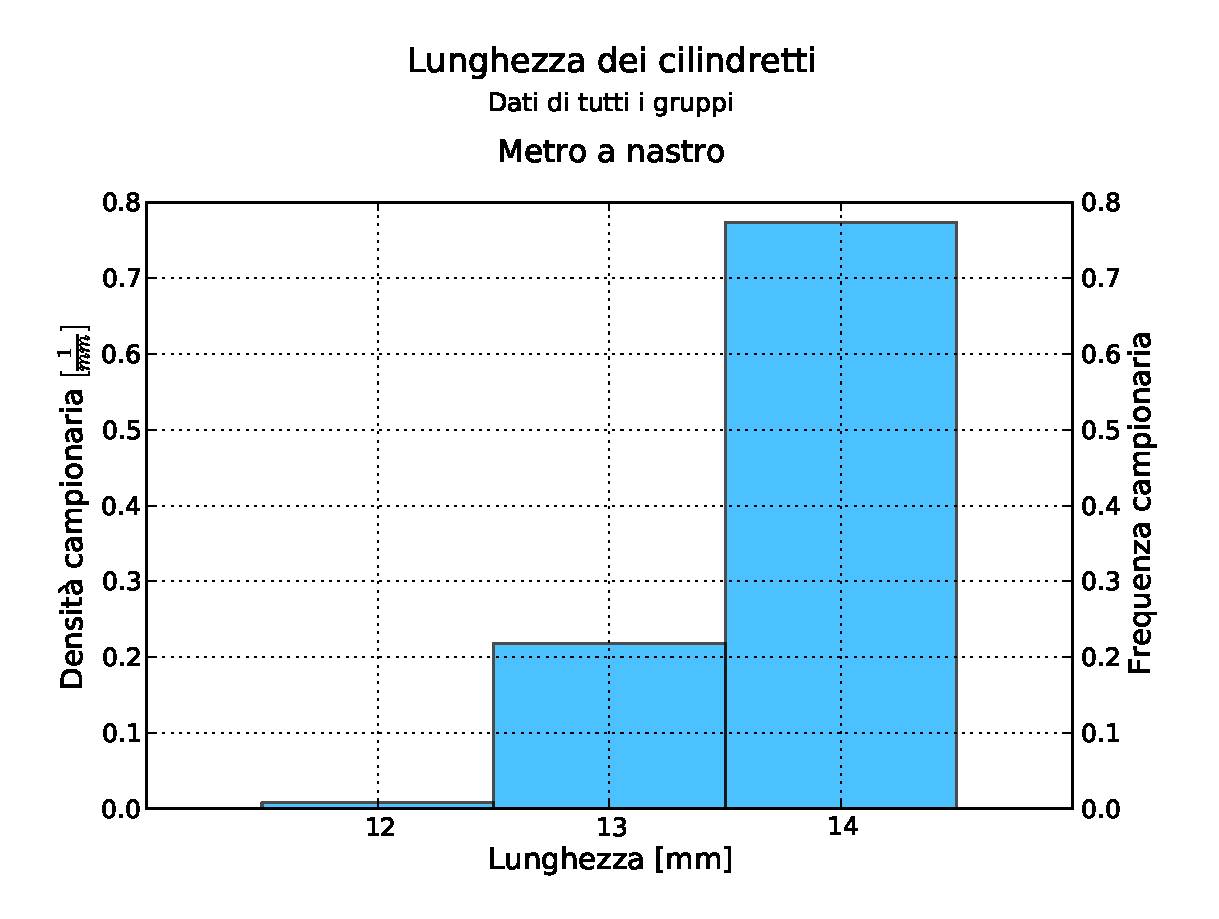
\includegraphics[width=100mm]{cilindri_tutti.pdf}
	\caption{Misure della lunghezza dei cilindretti ottenute da tutti i gruppi del
        laboratorio (gruppi del lunedì). L'istogramma riporta le misure effettuate con
        il metro a nastro.}
\end{SCfigure}

\begin{wrapfloat}{figure}{l}{0pt}
	\centering
	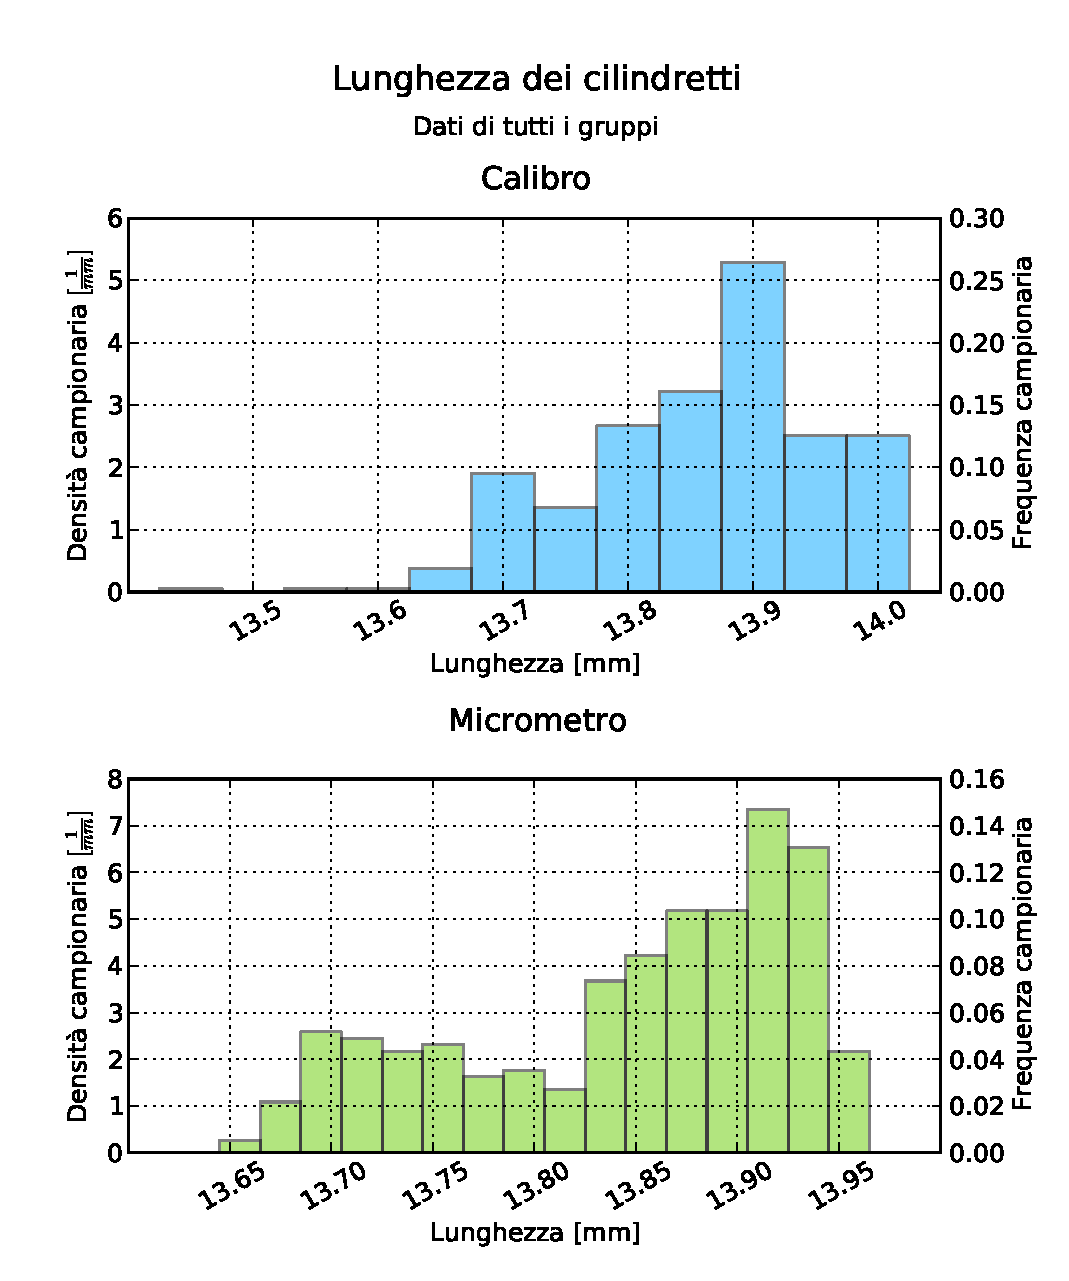
\includegraphics[width=100mm]{cilindri_tutti_2.pdf}
    \caption{Lunghezza dei cilindretti ottenute da tutti i gruppi (del lunedì)
        del corso di laboratorio. L'istogramma relativo alle misure con il calibro
        ha binning di 0.05 mm, mentre nell'istogramma delle misure effettuate con
        il micrometro i bin sono da 0.02 mm}
\end{wrapfloat}

\subsection{Analisi dei dati a livello globale di laboratorio}
Contrariamente a quanto abbiamo potuto osservare e ipotizzare tramite i dati
raccolti dal nostro singolo gruppo con i tre strumenti, unendo i dati relativi
a tutti i gruppi di laboratorio, si può evidenziare l'esistenza di due popolazioni
distinte di cilindri. Infatti nell'istogramma (1.3) sono ben distinguibili due picchi,
che corrispondono alle due rispettive medie campionarie di lunghezza delle due
popolazioni di cilindretti.



\newpage

\section{Pendolo}

La seconda parte di questa relazione tratta l'esperienza di misura del periodo
di un pendolo. Lo scopo dell'esperienza è imparare a trattare gli errori
casuali, dovuti alla procedura di misurazione del periodo con un cronometro,
che introduce inevitabilmente fluttuazioni casuali nelle misure effettuate,
e gli errori sistematici, dovuti alla diversa prontezza di riflessi degli
sperimentatori. In questo ultimo caso sorge il problema della 
compatibilità delle misure effettuate dai tre diversi membri del gruppo.

Ci siamo anche posti il problema di verificare sperimentalmente la
correttezza della legge del pendolo semplice, cosa che ogni studente di
fisica dovrebbe fare almeno una volta nella sua vita!

\subsection{Descrizione della procedura di misura}

\subsubsection{Apparato sperimentale}

Il pendolo è stato realizzato con un filo da pesca, che si può considerare
inestensibile, fissato con un morsetto al supporto del tavolo da laboratorio.
All'altra estremità del cavo è stato appeso, attraverso un gancio, un corpo
cilindrico di metallo di massa m = 205 g. Il pendolo si può schematizzare,
trascurando il gancio, come un cavo di lunghezza $l_c = 55.8 (???) \pm 0.2 \, (???)
cm$ unito ad un cilindro omogeneo di altezza $h = 5.1 \pm 0.05 \, cm$ (???).

\subsubsection{Predizione teorica (??? spostare? ???)}

Per il calcolo teorico del periodo è stato utilizzato il modello del pendolo
semplice, che abbiamo considerato adeguato alla situazione. La massa $m_c$ del
cavo è stata considerata trascurabile, o meglio poiché $m_c \ll m$ si è posto
$m_c = 0$. Inoltre, dato che in realtà
il cilindro non è puntiforme, lo abbiamo approssimato ad un punto
materiale posizionato nel suo baricentro, che si trova ad una distanza
$\frac{h}{2}$ dal punto di sospensione del corpo.
Nel modello del pendolo semplice, la lunghezza del cavo è quindi
$l = l_c + \frac{h}{2} = 55.8 \pm [] \, cm + 2.5 \pm [] \, cm = 58.3 \pm [] \, cm = 0.583 \pm [] \, m$.
Con questo valore di l e con $g = 9.8 \frac{m}{s^2}$ si ottene un periodo:

\begin{equation}
    \mathcal{T} = 2\pi \sqrt{\frac{l}{g}} = 1.499 \, s 
\end{equation}

Questo valore è quindi il valore atteso di periodo del pendolo. Lo scopo
dell'esperimento è quello di verificare sperimentalmente se questa predizione
è corretta.

%% da spostare più in giu??? forse sotto a "Processo di acquisizione dei dati sperimentali"?
\subsubsection{Errori sistematici (spostare???)}

Al fine di evitare errori sistematici riguardanti il modello teorico,
cioè errori causati dal fatto che il modello teorico non rispechia l'apparato
sperimentale usato, sono state prese le seguenti precauzioni:

\begin{itemize}
    \item{Si è tentato di contenere le oscillazioni del pendolo in un
        unico piano verticale. Abbiamo notato che a causa delle
        vibrazioni al momento del rilascio, il pendolo tende a seguire una
        traiettoria ellittica, invece che compiere la sua oscillazione su di un piano.
        Nei casi in cui la traiettoria si discostasse significativamente dal piano
        si è quindi proceduto a ripetere da capo la misura.}
    
    \item{Durante le operazioni di misura abbiamo mantenuto il massimo numero
        di oscillazioni entro il valore 20-30 affinché l'attrito con l'aria
        non influisse in modo significativo sul periodo del pendolo.}

    \item{Ci siamo accertati che l'ampiezza massima delle
        oscillazioni non superasse i 10$^\circ$ dalla verticale, in modo che
        l'approssimazione lineare $sin(\vartheta) \simeq \vartheta$ che viene
        utilizzata per calcolare la legge del pendolo sia accettabile. Infatti, per un
        angolo $\vartheta < 10^\circ = 0.175 \,\, rad$ si ha che:}

    \begin{equation}
        sin(\vartheta) = 0.174 \qquad \frac{\vartheta}{sin(\vartheta)} = 1.005
    \end{equation}

\end{itemize}

Possiamo stimare l'errore sistematico commesso ...

\begin{equation}
    \delta x_{sys} = 
\end{equation}

% Non so se questo è effettivamente interessante ai fini della discussione:
[Tramite il disegno dell'angolo massimo su un foglio di carta appositamente
posizionato vicino al punto di sospensione del filo.]

Tra gli errori sistematici segnaliamo, inoltre, il fatto che le misure sono state
effettuate da sperimentatori diversi, che introducono degli errori sistematici
che variano da persona a persona. Questi errori saranno trattati nella sezione
di analisi dei dati.

%% frase un po' scema???
Le precauzioni prese dovrebbero essere sufficienti a ridurre l'errore sistematico
entro limiti accettabili. Tuttavia è risaputo che gli errori sistematici
sono i più difficili da scovare ed eliminare.
	
\begin{table}[bt]
	\begin{tabular} {c c c c | c c c c | c c c c}
		\toprule
		\multicolumn{12}{c}{Periodo del pendolo [s]} \\
		\multicolumn{4}{c}{Francesco} & \multicolumn{4}{c}{Davide} & \multicolumn{4}{c}{Andrea} \\
		\midrule
		15.04 & 14.99 & 14.99 & 14.97 & 14.91 & 14.97 & 15.06 & 15.04 & 14.98 & 14.98 & 15.05 & 15.01 \\
		14.99 & 14.99 & 15.01 & 15.08 & 14.92 & 15.06 & 15.08 & 15.02 & 14.85 & 14.99 & 14.98 & 15.00 \\
		15.04 & 15.00 & 15.06 & 14.98 & 15.06 & 15.02 & 15.04 & 15.00 & 15.04 & 14.99 & 14.99 & 14.94 \\
		14.93 & 14.98 & 14.98 & 15.04 & 15.06 & 15.06 & 15.02 & 14.91 & 15.01 & 15.00 & 15.13 & 14.99 \\
		14.99 & 14.91 & 15.03 & 15.03 & 15.03 & 15.02 & 15.06 & 15.02 & 14.88 & 15.01 & 15.02 & 14.96 \\
		\bottomrule
	\end{tabular}

	\caption{Tabella delle misure del periodo del pendolo ottenute dai 3 membri del gruppo.
        Ogni sperimentatore ha raccolto 20 misure di 10 periodi. Sono riportati
        i dati grezzi di lettura del cronometro, riferiti a 10 periodi. }
\end{table}

\subsubsection{Processo di acquisizione dei dati sperimentali}

Per le misurazioni è stato utilizzato un comune cronometro con risoluzione di
misura pari a 0.01 s. [errore di risoluzione???] Ogni componente del gruppo ha
cronomerato 20 volte il tempo impiegato dal pendolo per compiere 10 periodi.
I valori grezzi misurati, riportati nella tabella 2, sono stati divisi per
10 per ottenere il valore medio del periodo del pendolo. Questo ci ha permesso
di diminuire gli errori sistematici dovuti alla prontezza di riflessi dei diversi
operatori, che verranno trattati più approfonditamente della sezione di analisi dei
dati, e di aumentare la risoluzione del cronometro fino a 1 millisecondo.

Successivamente un componente del gruppo ha eseguito 100 misurazioni di periodi
singoli dell'apparato, riportate nella tabella 3. L'aquisizione di dati è stata
effettuata con la seguente procedura:

% si può forse togliere l'elenco???
\begin{enumerate}
    \item{Il pendolo è stato fatto oscillare prestando attenzione al piano di oscillazione
        e all'ampiezza dell'oscillazione.}

    \item{Si è misurato un periodo, annotato il valore ottenuto e azzerato il cronometro.}

    \item{Le misurazioni sono state intervallate da 1-2 periodi non misurati.}

    \item{Ogni 10 misurazioni, che equivale a meno di 30 periodi, il pendolo è stato fermato
        e fatto ripartire, per evitare lo smorzamento dovuto all'attrito con l'aria.}
\end{enumerate}

Non è stato utilizzata la funzione «giro» del cronometro, al fine di evitare
di introdurre dipendenza tra le varie misure. Azzerando il cronometro ogni 
volta le misure risultano statisticamente indipendenti.

\begin{SCtable}[][bt]
	\centering
	\begin{tabular} {c c c c c | c c c c c}
		\toprule
		\multicolumn{10}{c}{Periodo del pendolo - Misure di un operatore [s]} \\
		\midrule
		1.46 & 1.54 & 1.55 & 1.57 & 1.41 & 1.45 & 1.52 & 1.45 & 1.37 & 1.53 \\
		1.57 & 1.50 & 1.52 & 1.50 & 1.48 & 1.49 & 1.44 & 1.49 & 1.43 & 1.53 \\
		1.50 & 1.50 & 1.56 & 1.61 & 1.45 & 1.38 & 1.52 & 1.41 & 1.60 & 1.49 \\
		1.48 & 1.53 & 1.52 & 1.55 & 1.54 & 1.46 & 1.51 & 1.51 & 1.49 & 1.52 \\
		1.52 & 1.50 & 1.48 & 1.46 & 1.41 & 1.48 & 1.45 & 1.48 & 1.52 & 1.51 \\
		\midrule
		1.55 & 1.52 & 1.55 & 1.49 & 1.51 & 1.50 & 1.52 & 1.49 & 1.54 & 1.52 \\
		1.45 & 1.49 & 1.47 & 1.47 & 1.48 & 1.48 & 1.53 & 1.51 & 1.52 & 1.47 \\
		1.54 & 1.42 & 1.43 & 1.45 & 1.49 & 1.42 & 1.47 & 1.36 & 1.50 & 1.55 \\
		1.58 & 1.52 & 1.45 & 1.48 & 1.44 & 1.52 & 1.51 & 1.50 & 1.54 & 1.52 \\
		1.52 & 1.52 & 1.47 & 1.52 & 1.44 & 1.56 & 1.50 & 1.49 & 1.52 & 1.56 \\
	\bottomrule
	\end{tabular}
	\caption{Misure di periodo effettuate da uno dei tre componenti del gruppo.
        Sono riportati i valori di lettura del cronometro riferiti a singole oscillazioni
        (periodi) dell'apparato.}
\end{SCtable}

\subsection{Analisi dei dati}

La Tabella 1 e la Figura 1 (l'istogramma) riguardano la distribuzione dei dati
relativi la misura del singolo periodo del pendolo da parte di tutti e tre i
componenti del gruppo.

\begin{figure}[][p]
	\centering
	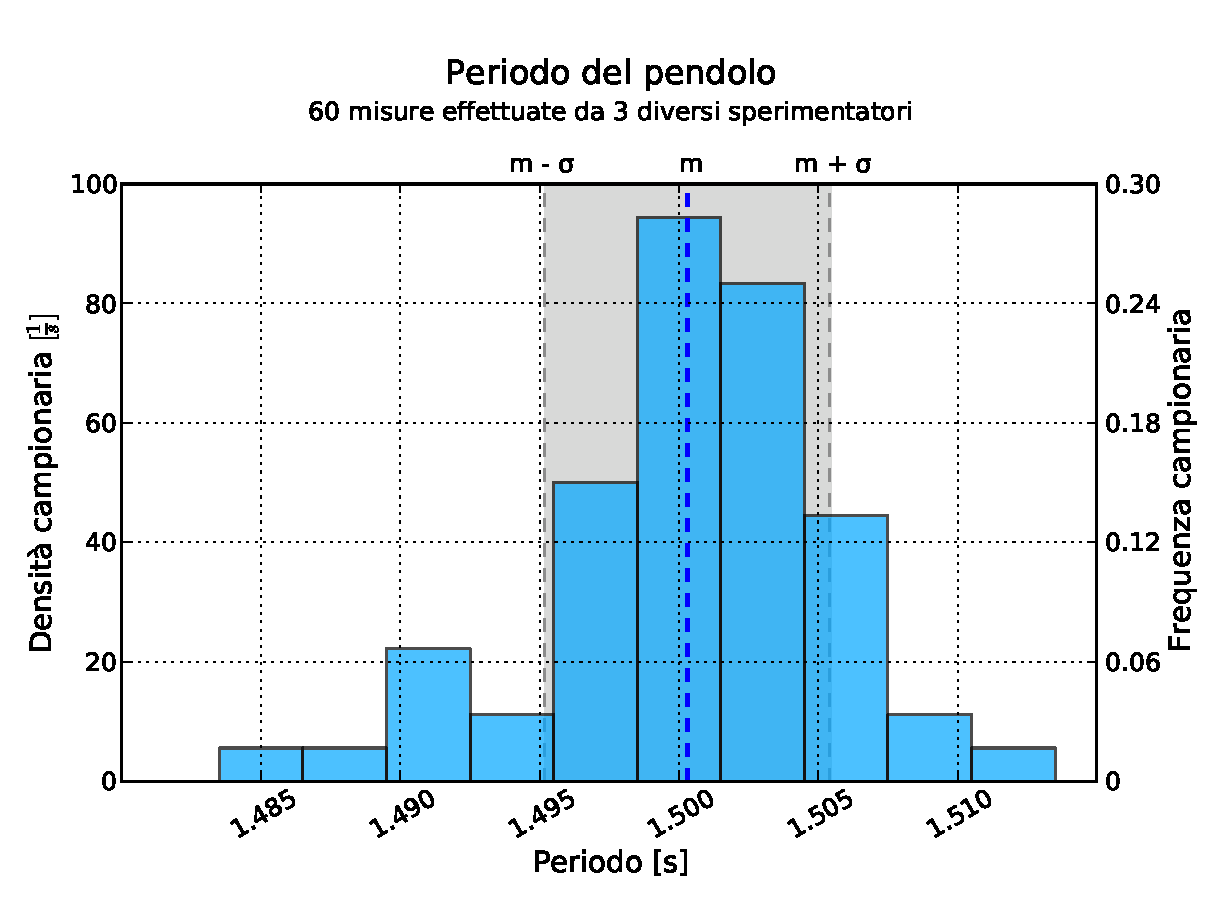
\includegraphics[width=120mm]{Pendolo.pdf}
	\caption{Istogramma relativo alle misure effettuate da tutti e tre gli sperimentatori}
\end{figure}

\begin{figure}[][p]
	\centering
	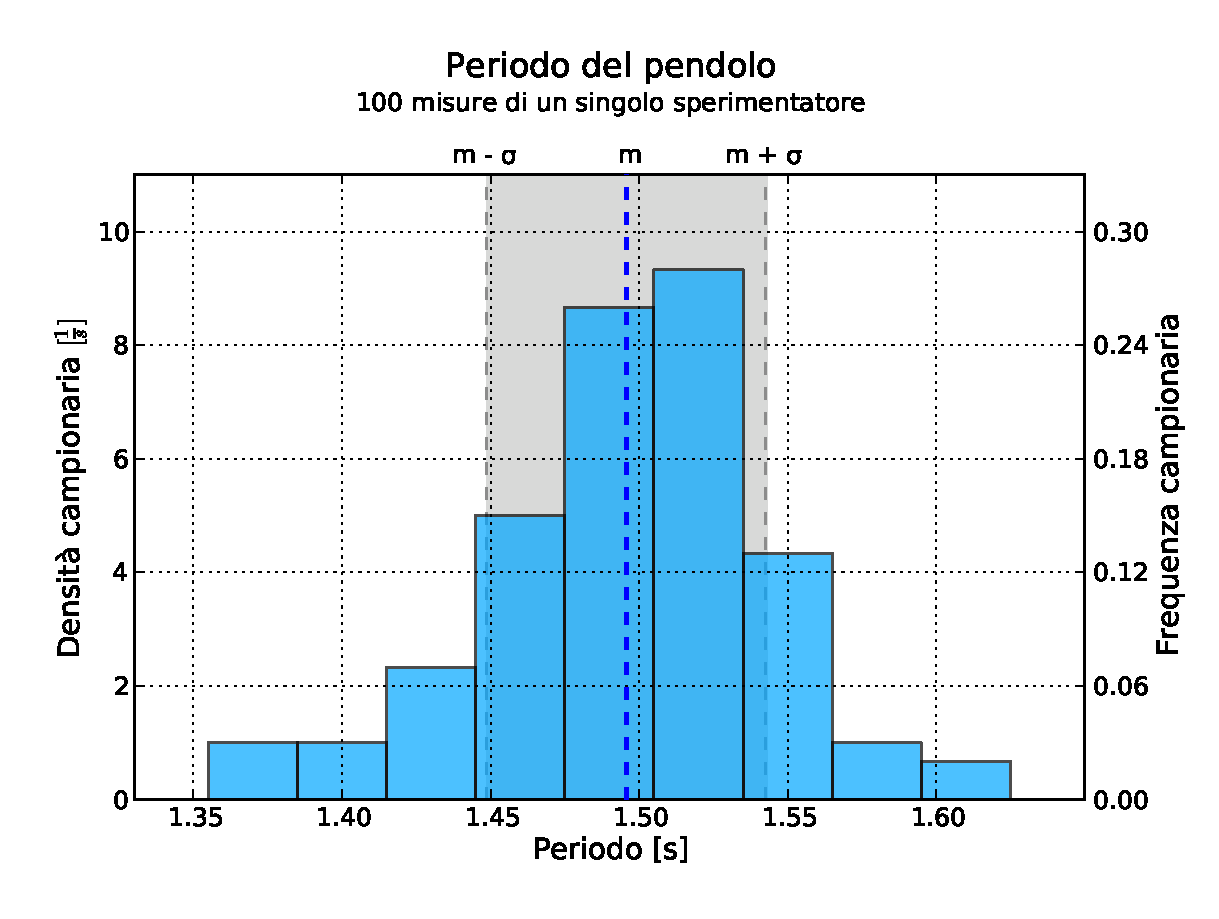
\includegraphics[width=120mm]{Pendolo100.pdf}
	\caption{Istogramma delle 100 misure singole di periodo}
\end{figure}

\begin{figure}[bt]
	\centering
	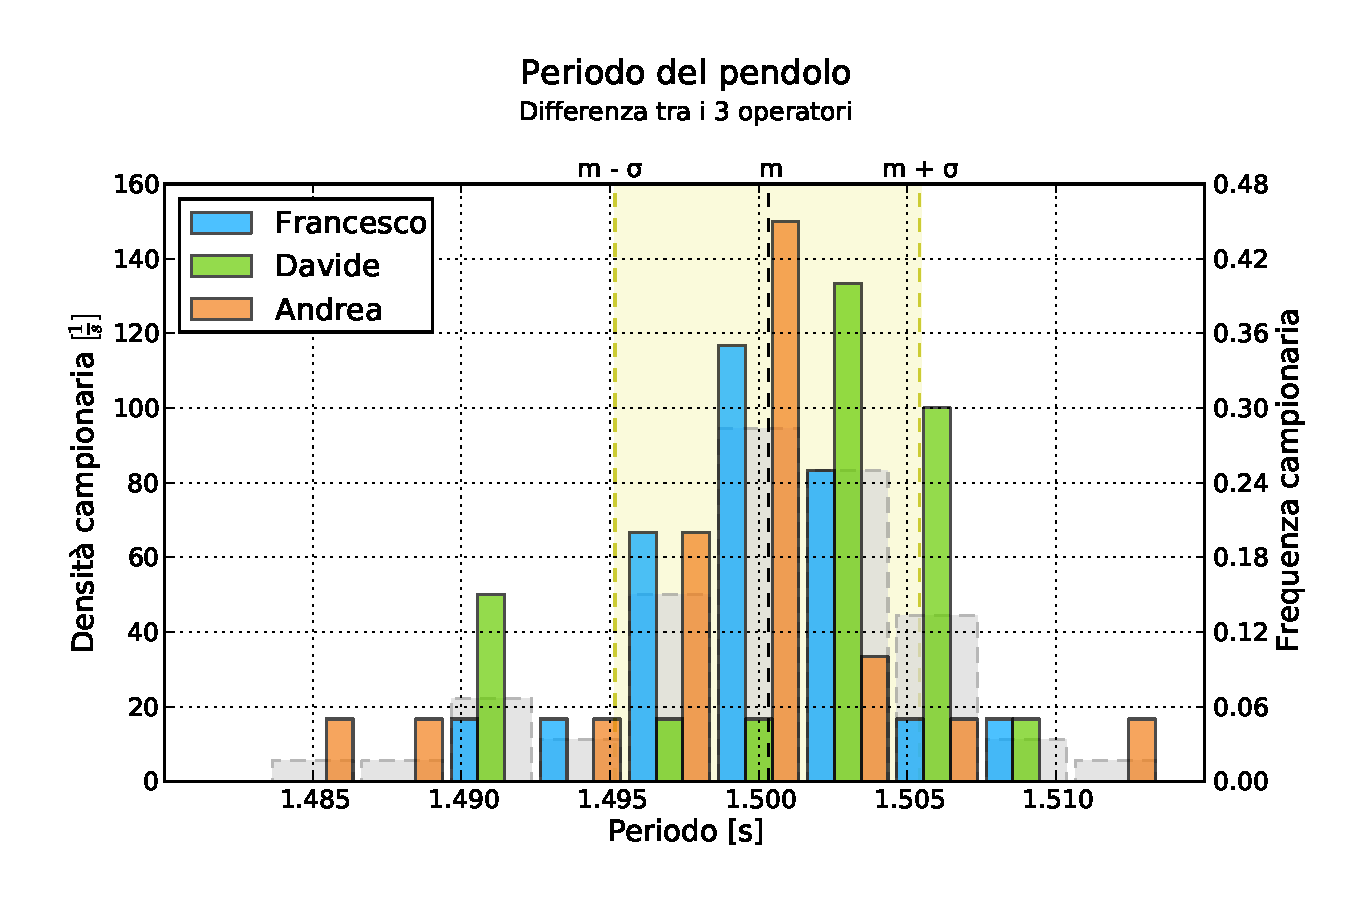
\includegraphics[width=150mm]{pendolo3.pdf}
	\caption{didascalia}
\end{figure}

Analizzando parzialmete i dati sopra riportati possiamo ricavare che la media
camponaria e gli altri parametri della distribuzione dei dati relativi a
ogni singolo sperimentatore sono:

\begin{equation*}
	\begin{split}
		m_{Francesco}^* = 1.500\,s \pm 0.004\,s \\
		m_{Davide}^* = 1.502\,s \pm 0.005\,s \\
		m_{Andrea}^* = 1.499\,s \pm 0.006\,s
	\end{split}
\end{equation*}
\begin{equation*}
	\begin{split}
		\tilde{\sigma}_{Francesco} = 0.004\,s \\
		\tilde{\sigma}_{Davide} = 0.005\,s \\
		\tilde{\sigma}_{Andrea} = 0.006\,s \\
		\tilde{\sigma}_{ris-std} = 0.0003\,s
	\end{split}
\end{equation*}\\

[Le misure sono COMPATIBILI ?????????]\\

Le misure ripetute del periodo di un pendolo mostrano che le fluttuazioni
delle misure sono dovute principalmente ad errori casuali, poichè il periodo
$\mathcal{T}$ di oscillazione di un pendolo semplice è isocrono per ampiezze
di oscillazioni abbastanza piccole, nel nostro caso contenute entro i dieci gradi.
Per questo motivo è importante sottolineare che l'incertezza standard sulla
misura del perido risulta essere molto minore (circa dieci volte) dell'incertezza
dovuta a errori di tipo A, quindi terremo conto principalmente di quest'ultima.

Procedimo ora con l'analisi complessiva dei dati relativi alla misura del
periodo del pendolo eseguita da tutti e tre i componenti del gruppo e otteniamo che:

% se vuoi elenco numerato sostituisci enumerate al posto di itemize
% ovviemente devi cambiare anche \end{itemize}
\begin{itemize}
    \item{La media campionaria é:}
        \begin{equation}
            m^*[\mathcal{T}] = \frac{1}{N} \sum_{i=1}^{N} \mathcal{T}_i = 1.500\,s
        \end{equation} 

    \item{La varianza campionaria del periodo di oscilazione del pendolo è:}
        \begin{equation}
            \tilde{D}[\mathcal{T}] = \frac{1}{N - 1} \sum_{i=1}^{N} (\mathcal{T}_i - m^*[\mathcal{T}])^2 = 0.00003\,s
        \end{equation}

    \item{la deviazione standard campionaria risulta essere:}
        \begin{equation}
            \tilde{\sigma}[\mathcal{T}] = \sqrt{\frac{1}{N - 1} \sum_{i=1}^{N} (\mathcal{T}_i - m^*[\mathcal{T}])^2} = 0.005 s
        \end{equation}

    \item{la mediana, il quantile 10\% e il quantile 90\% sono relativamente:}
        \begin{equation*}
            m = 1.501\,s \quad
            q_{10\%} = 1.493\,s \quad
            q_{90\%} = 1.506\,s
        \end{equation*}
\end{itemize}

Pertanto, applicando le necessarie approssimazioni e gli errori relativi ad ogni misura si ottiene
\begin{equation*}
m^*[\mathcal{T}] = 1.500 \pm 0.005\,s
\end{equation*}
\begin{equation*}
m = 1.500 \pm 0.005\,s  \quad
q_{10\%} = 1.495 \pm 0.005\,s \quad
q_{90\%} = 1.505 \pm 0.005\,s
\end{equation*}

Come si può notare dall'analisi fatta non abbiamo riscontrato particolari errori sistematici dovuti all'operatore, in quanto la media campionaria dei dati di ogni operatore è compatibile con la media di tutti i valori entro la deviazione standard campionaria. Inoltre se le misure di uno sperimentatore fossero state affette da un errore sistematico i suoi valori medi sarebbero risultati significativamente differenti da quelli degli altri due componenti del gruppo.
Come si può notare dagli istogrammi sono invece evidenti gli errori casuali. Ciononostante il loro valore è contenuto grazie al fatto che abbiamo deciso di misurare il periodo di 10 oscillazioni consecutive.\\
Quindi grazie hai risultati così ottenuti possiamo dire che il periodo del pendolo risulta essere:

\begin{equation}
\mathcal{T} = \mathcal{T}_0 \pm \delta\mathcal{T} = 1.500\,s \pm 0.005\,s
\end{equation}\\

\newpage

La Tabella 2 e la Figura 2 invece sono relativi alla misura del periodo del pendolo da parte di un singolo membro del gruppo.


Procediamo ora con l'analisi dei dati relativi alle cento misurazioni del periodo:

% se vuoi elenco numerato sostituisci enumerate al posto di itemize
% ovviemente devi cambiare anche \end{itemize}
\begin{itemize}
    \item{la media campionaria é:}
        \begin{equation}
            m^*[\mathcal{T}] = \frac{1}{N} \sum_{i=1}^{N} \mathcal{T}_i = 1.50\,s
        \end{equation} 

    \item{la varianza campionaria del periodo di oscilazione del pendolo è:}
        \begin{equation}
            \tilde{D}[\mathcal{T}] = \frac{1}{N - 1} \sum_{i=1}^{N} (\mathcal{T}_i - m^*[\mathcal{T}])^2 = 0.0022\,s
        \end{equation}

    \item{la deviazione standard campionaria risulta essere:}
        \begin{equation}
            \tilde{\sigma}[\mathcal{T}] = \sqrt{\frac{1}{N - 1} \sum_{i=1}^{N} (\mathcal{T}_i - m^*[\mathcal{T}])^2} = 0.05\,s
        \end{equation}

        \begin{equation}
            \tilde{\sigma}_{ris-std} = 0.003\,s
        \end{equation}

    \item{la mediana, il quantile 10\% e il quantile 90\% sono relativamente:}
        \begin{equation*}
            m = 1.50\,s \quad
            q_{10\%} = 1.44\,s \quad
            q_{90\%} = 1.55\,s
        \end{equation*}
\end{itemize}

Innanzitutto, si può notare che le cento misure di oscillazione di un singolo periodo hanno una precisione fino al centesimo di secondo, mentre quelle relative a tutti e tre i componenti avevano una precisione fino al millesimo. Infatti la deviazione standard di queste misure è di un ordine di grandezza maggiore rispetto al dato relativo alle misure precedenti.\\
Se procediamo ora con un'analisi più approfondita dei dati e li raggruppiamo in dieci gruppi di dieci misure ciascuno, possiamo calcolare la media campionaria di ogni singolo gruppo:

\begin{equation}
m_k^* \quad con \,\, K \in{\{1,2,...,10\}}
\end{equation}

dove k indica il numero del gruppo considerato.
Ottenute queste misure possiamo considerarle come singoli dati e farne una media campionaria ($ m[m_k^*] $):

\begin{equation}
m[m_k^*] = \sum_{k=1}^{10} (m_k^*) = 1.50\,s
\end{equation}

che risulta essere uguale alla media campionaria delle cento misure prese singolarmente. Calcolando la deviazione standard delle medie ($ \sigma[m_k^*] $):

\begin{equation}
\sigma[m_k^*] = \sqrt{\frac{10}{10-1} \sum_{k=1}^{10} (m_k^* - m[m_k^*])^2} = 0.020\,s
\end{equation}

otteniamo che il rapporto tra $\frac{\tilde{\sigma}[\mathcal{T}]}{\sigma[m_k^*]}$ risulta essere circa 0.42 che è un risultato attendibile dal momento che la predizione teorica ci dice che:

\begin{equation}
\frac{\tilde{\sigma}[\mathcal{T}]}{\sigma[m_k^*]} = \frac{1}{\sqrt{10}} \simeq \, 0.32
\end{equation}








\newpage

\section{Conclusioni}
[i cilindretti fanno cacare]



\begin{equation}
\tilde{D} = \frac{1}{N - 1} \sum_{i=1}^{N} (x_i - m^*[x])^2
\end{equation}

\begin{equation}
\tilde{\sigma} = \sqrt{\frac{1}{N - 1} \sum_{i=1}^{N} (x_i - m^*[x])^2}
\end{equation}

\begin{equation}
m^*[x] = \frac{1}{N} \sum_{i=1}^{N} (x_i) \simeq \sum_{j=1}^{\mathcal{N}} (x_j p_j^*) 
\end{equation}

\begin{equation}
p_j^* = \frac{n_j^*}{N} 
\end{equation}

\begin{equation}
f_j^* = \frac{n_j^*}{N\Delta x}
\end{equation}

\begin{equation}
D^* = \langle(x - m^*)^2\rangle = \frac{1}{N} \sum_{i=1}^{N} (x_i - m^*[x])^2
\simeq \sum_{j=1}^{\mathcal{N}} (x_j - m^*)^2 p_j^*)
\end{equation}

\begin{equation}
m^*[\mathcal{T}] = \frac{1}{N} \sum_{i=1}^{N} \mathcal{T}_i
\end{equation}

\begin{equation}
\sigma^*[\mathcal{T}] = \sqrt{\frac{1}{N} \sum_{i=1}^{N} (\mathcal{T}_i - m^*)^2}
\end{equation}

\begin{equation}
\mathcal{T} = \mathcal{T}_0 \pm \delta\mathcal{T}
\end{equation}

\begin{equation}
\mathcal{T}_0 = m^* = \frac{1}{N} \sum_{i=1}^{N} \mathcal{T}_i
\end{equation}

\begin{equation}
\delta\mathcal{T}_{cas} = \tilde{\sigma}[m^*] = \frac{1}{\sqrt{N}} \sqrt{\frac{N}{N - 1}}\sigma^*[\mathcal{T}] = \sqrt{\frac{1}{N(N - 1)} \sum_{i=1}^{N} (\mathcal{T}_i - m^*)^2}
\end{equation}

\end{document}
